\begin{frame}{Reconhecimento de Voz}{Definição e componentes básicas}

\begin{block}{Definição}
\emph{Reconhecimento automático de voz} é um campo voltado ao desenvolvimento de técnicas para que computadores possam captar, reconhecer e traduzir a linguagem falada para texto
\end{block}

\uncover<2->{
\begin{figure}
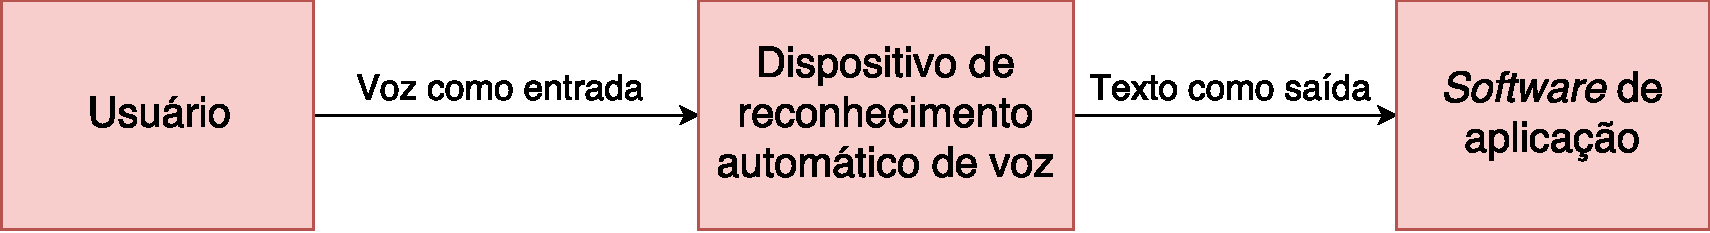
\includegraphics[width=\textwidth]{image/generic-stt.pdf}
\end{figure}
}

\end{frame}
